\section{WR}

\subsection{Theory}
%what is WR

WR, short for weighted random, is one of the two settings used for rounding in kill-rates. While in the section for kill-rates I referred to SR 0\% luck as deterministic settings, WR works in a different way, where when you perform a an attack of 3 armies against a 2 army neutral, the outcome is based on Probabilities.
\\
\\
For each attack the game computes $E=\text{armies} \times \text{kill-rate}$ then turns that fractional expectation E into a whole number of kills with a single, biased coin-flip. In a 4vs3 scenario, $4\times 0.6 = 2.4$ results in 60\% chance to kill 2 defenders and 40\% chance to kill 3 defenders. WR never gives "wild roles" that are 2-3 more values away from the expectation, it's outcome comes at $\pm 0.8$ variance at most.
\\
\\
WR templates are played in a completely different style than WR ones, and although the principles you know and apply in SR are universal, the game here revolves more around knowing when to take a risk and when not to. You'll find that a lot of WR templates resort to including RMO, as a why that balances out the luck aspect of the game, as in "you can get lucky with WR, but your opponent can get lucky with RMO".

\subsection{Templates}

There are currently ten different WR templates in the MTL, with six out of those having all around the same settings but different map dynamics and cards. These templates are in Table \ref{table:wr_overview}.

%--------------- Weighted-Random templates (sorted by Arm/Init, then Income) ---------------
\scriptsize
\begin{longtable}{|l|c|c|c|c|c|c|c|c|}
\hline
\rowcolor{Baby_Blue}
Template & Move & Init & Arm/\newline Init & Neutr & Neutr in & Wastes & Waste & Income \\ 
\rowcolor{Baby_Blue}
(Name)   & order& terr & terr            & Size  & Dist      & (\#)   & Size  & (base) \\ \hline\hline
\endfirsthead
\hline
\rowcolor{Baby_Blue}
Template & Move & Init & Arm/\newline Init & Neutr & Neutr in Dist & Wasts & Waste sz & Income \\ \hline\hline
\endhead
% ---- Arm/Init = 6 ----------------------------------------------------------
Belarus                 & cycle  & 3 & 6 & 3 & 2 & 35 & 2  & 5 \\ \hline
% ---- Arm/Init = 5 ----------------------------------------------------------
Great Lakes             & cycle  & 4 & 5 & 3 & 2 & 15 & 4  & 6 \\ \hline
% ---- Arm/Init = 4 | Income = 5 --------------------------------------------
British Raj             & random & 4 & 4 & 2 & 2 & 7  & 12 & 5 \\ 
Randomized Strat ME     & random & 3 & 4 & 2 & 4 & 7  & 10 & 5 \\ 
Strat ME                & random & 3 & 4 & 2 & 4 & 7  & 10 & 5 \\ 
Phobia                  & random & 3 & 4 & 2 & 4 & 6  & 10 & 5 \\ 
Final Fantasy VII       & random & 3 & 4 & 2 & 4 & 6  & 10 & 5 \\ 
Tor-ture                & random & 4 & 4 & 2 & 4 & 6  & 10 & 5 \\ 
% ---- Arm/Init = 4 | Income = 4 --------------------------------------------
Strategic Commanders    & cycle  & 3 & 4 & 3 & 5 & 7  & 10 & 4 \\ \hline
% ---- Arm/Init = 2 ----------------------------------------------------------
Pangea Ultima           & cycle  & 3 & 2 & 2 & 4 & 8  & 10 & 6 \\ \hline
\caption{Weighted-Random templates order on Armies per Initial Territory and Income}
\label{table:wr_overview}
\end{longtable}
\normalsize


\subsection{Probabilities \& Expanding Efficiently}
% for scenarios

While in SR there are strict income transitions principles, WR is more about probabilities. As it is rather time consuming to calculate probabilities, I will give you in this section some of the different scenarios as well as the way to optimize your moves as fast as possible. 
\\
\\
Consider the scenario of a single pick in a central territory of a +3 bonus in a template like Strat ME as in Antarctica in this \href{https://www.warzone.com/MultiPlayer?GameID=13172709}{game} and Image \ref{3bonus_ftb_wr}. This un-intuitive idea is theoretically possible, just not probable, in Strat ME. Since you have to que three attacks of 3/3/2 on Turn 1 in order to finish the bonus, all three must succeed.
\begin{itemize}
    \item 3vs2, 3 attackers capture 2 neutrals $3 \times 0.6 = 1.8 \rightarrow 80\%$ of the time.
    \item 2vs2, 2 attackers capture 2 neutrals $ 2 \times 0.6 = 1.2 \rightarrow 20\%$ of the time.
\end{itemize}

For all three to succeed, $P = P_3 \times P_3 \times \times P_2 = 0.8 \times 0.8 \times 0.2 = 0.128$ or \textbf{12.8\%}.

\begin{figure}[H]
  \centering
  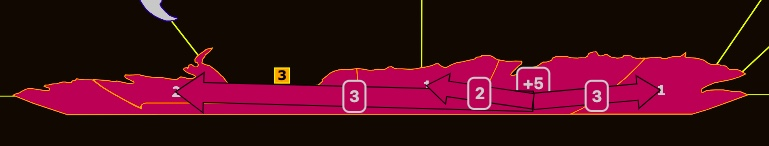
\includegraphics[width=0.7\textwidth]{Images/loveant.jpg}
  \caption{+3 FTB in WR}
  \label{3bonus_ftb_wr}
\end{figure}

We can extend this idea to completing a +4 bonus in Strat ME either in one or in two turns with a single pick. The possible sequences you can follow are:
\begin{enumerate}
    \item 4x +2 attacks on Turn 1
    \item Single +8 attack on Turn 1 into 3 attacks Turn 2
    \item Split Turn 1 into attacks of 3\&5 
    \item Split Turn 1 into attacks of 4\&4
\end{enumerate}

\textbf{4x +2 attacks on Turn 1}

If you do this I suggest uninstalling the game and converting to roulette. But if you do decide to do it, the probability to finish the bonus comes at $0.2^4$ or 0.16\%.
\\
\\
\textbf{Single +8 attack on Turn 1 into 3 attacks Turn 2}

To track the overall chance to finish the bonus following this sequence, as per Figure \ref{wrsc1}:

\begin{itemize}
    \item On Turn 1 we lose 1 attacker -> 6 movable left (60\%). Turn 2 we do 4/4/3 attacks, that's 80\% chance all three succeed (capture). Overall $0.6 \times 0.8 = 0.48$ -> 48\% chance to complete bonus.
    \item On Turn 1 we lose 2 attackers -> 5 movable left (40\%). Turn 2 we need 4/3/3 attacks to finish bonus, that's $0.8 \times 0.8 = 0.64$ chance those two attacks succeed (capture). Overall $0.4 \times 0.8 \times 0.8 =0.256$ -> 25.6 \% chance to complete bonus.
    \item Adding the 2 different scenarios together, there's an overall \textbf{73.6 \%} chance of finishing the bonus on Turn 2.
\end{itemize}

\begin{wrapfigure}{r}{0.35\textwidth}
    \centering
    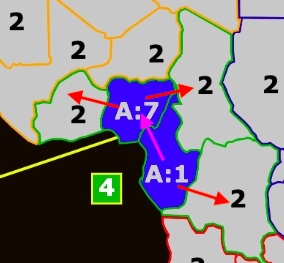
\includegraphics[width=0.25\textwidth]{Images/wrsc1.jpg}
    \caption{Single attack of 8. Losing either 1 or 2 attackers (in the picture 1). Requiring three attacks on Turn 2}
    \label{wrsc1}
\end{wrapfigure}

\textbf{Split Turn 1 into attacks of 3 \& 5}

This is a rather more complicated calculation that I try to simplify in Figure \ref{wrprob_35}.

\begin{enumerate}
    \item On turn 1, two attacks are queued, a 5vs2 and a 3vs2 attack. 
    \begin{itemize}
        \item 5vs2 always works, 60\% for -1 attacker, 40\% for -2 attackers
        \item 3vs2 doesn't work always. In fact the probabilities are given at the top of the graph for the attack
\[
\left\{
\begin{aligned}
P(C \land L_{1}) &= 0.48 \\[4pt]
P(C \land L_{2}) &= 0.32 \\[4pt]
P(\bar{C} \land L_{1}) &= 0.12 \\[4pt]
P(\bar{C} \land L_{2}) &= 0.08
\end{aligned}
\right.
\]
where C denotes capturing the neutral, $\bar{C}$ denotes not capturing the neutral, and $L_k$ the number of attackers lost. For example for Not capturing the neutral (20\%) and losing 2 attackers (40\%), overall probability comes at $0.2\times 0.4$ 
    \end{itemize}
    \item After Turn 1, there are 8 scenarios and different approaches on Turn 2, as in Figure \ref{wrprob_35}.
    \item It can be counted that the overall success probability comes at \textbf{94.368 \%} and chance to fail at \textbf{5.632 \%}.
\end{enumerate}

\begin{figure}[H]
  \centering
  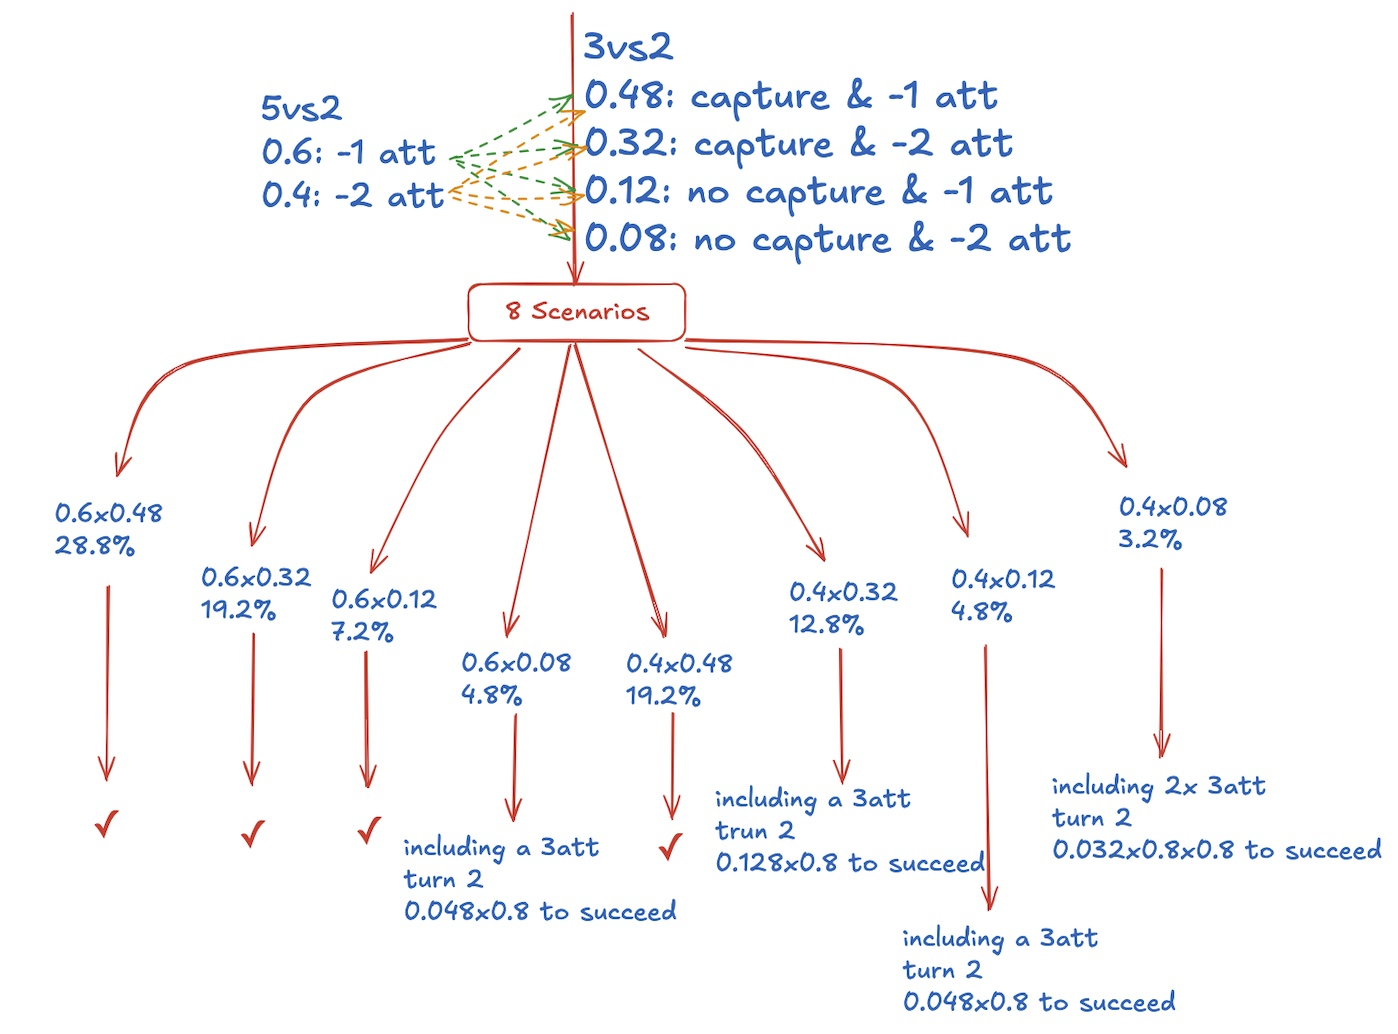
\includegraphics[width=0.7\textwidth]{Images/wr_probabilitie.jpg}
  \caption{Probability tree for doing split attacks of 3 and 5 Turn 1}
  \label{wrprob_35}
\end{figure}

If it helps at understanding when completing the 4bonus can fail, denoting as b1-b8 from left to right the scenarios above:
\begin{itemize}
    \item b1: -1 attacker from 5vs2 and 0.48 scenario from 3vs2 (capture and -1 attacker). b1 comes at $0.6\times0.48 = 0.288 \rightarrow 28.8\%$ of the times. Can always finish bonus with 2x 4vs2 attacks
Similarly, 
    \item b2: $0.6\times0.32 = 0.192$, always have enough to finish bonus on Turn 2
    \item b3: $0.6\times0.12 = 0.072$ always have enough to finish bonus on Turn 2
    \item b4: $0.6\times0.08=0.048$. Attack of 3vs2 has failed and we lost 2 attackers, so we need +1 deployed to get the now 1army neutral with a 2attack. Besides that we have +1 deployed for a 4army attack and +3 deployed for a 3army attack. Risk involved. In this subscenario 80\% of the time we complete bonus, 20\% we don't (due to the 3attack). Chance to fail at $0.048\times0.2 =0.0096$.
    \item b5: $0.4\times0.48 = 0.192$, Turn 2 we deploy 2+3, always enough to finish bonus
    \item b6: $.04\times0.32 = 0.128$, need a 3attack on turn 2, so $0.128\times0.2 = 0.0256$ chance to fail.
    \item b7: $0.4\times0.12 = 0.048$, need a 3attack on turn 2, so $0.048\times0.2 = 0.0096$ chance to fail.
    \item b8: $0.4\times0.08 = 0.032$, need two 3attacks on turn 2, so $0.032\times (1- (0.8\times0.8))=0.01152$ chance to fail. 
\end{itemize}

Overall chance to fail at adding b4, b6, b7, b8 at 5.632 \%.


\textbf{Split Turn 1 into attacks of 4\&4}

Following the same logic, 
\begin{enumerate}
    \item Two attacks of 4vs2 occur on Turn 1. Each attack always captures but comes at 60\% chance of having -1 attacker and 40\% chance of having -2 attackers.
    \item As a result there are three scenarios:
    \begin{itemize}
        \item c1: $0.6\times0.6 = 0.36$ or 36\% of the times we lose -1 attacker on each attack. In this scenario, we always have enough armies to finish bonus on Turn 2 (2+2 deployed a 1 elsewhere).
        \item c2: $0.6\times0.4\times2  = 0.48$ or 48\% of the times we lose -1 attacker on one and -2 attackers on the other attack. In this scenario, we always have enough armies to finish bonus on Turn 2 (2+3 deployed).
        \item c3: $0.4\times0.4 = 0.16$ or 16\% of the times we lose -2 attackers on each attack. In this scenario, we have to gamble at least one 3 attack to finish the bonus. Chance to fail comes at $0.16\times 0.2 = 0.032 \rightarrow 3.2\%$. 
    \end{itemize}
\end{enumerate}

To sum up all the above calculations, you can take four approaches of completing a +4 Bonus in Strat ME or it's clones, (Scenario 1 is as an FTB, Scenarios 2-4 for Completing it by the end of Turn 2), with the results in Table \ref{table:bonus_break_probs}.

%--------------- Break-probability overview (fill in numbers) ---------------
\begin{longtable}{|l|c|c|}
\hline
\rowcolor{Baby_Blue}
Attack plan (Turn-sequence) & Success prob.\ (\%) & Failure prob.\ (\%) \\ \hline\hline
\endfirsthead
\hline
\rowcolor{Baby_Blue}
Attack plan & Success prob.\ (\%) & Failure prob.\ (\%) \\ \hline\hline
\endhead
4 × +2 attacks on T1                & 0.16\% & 99.84 \% \\ \hline
+8 attack on T1 → 3 attacks on T2   & 73.6\% & 26.4\% \\ \hline
Split T1 into 3 \& 5 attacks         & 94.368 \% & 5.632 \% \\ \hline
Split T1 into 4 \& 4 attacks         & 96.8\% & 3.2 \% \\ \hline
\caption{Success / failure probabilities for alternative bonus-capture lines of a +4 bonus in Strat ME clones.}
\label{table:bonus_break_probs}
\end{longtable}

Use the methodology above in whichever scenario comes up to calculate the optimal way of expanding in whichever template/distribution you are playing. All that really matters is understanding why "more attacks" is a beneficial thing (example in Figures \ref{44wrsplit} and \ref{single8wr}).

\begin{figure}[H]
  \centering
  \begin{minipage}[b]{0.48\linewidth}
    \centering
    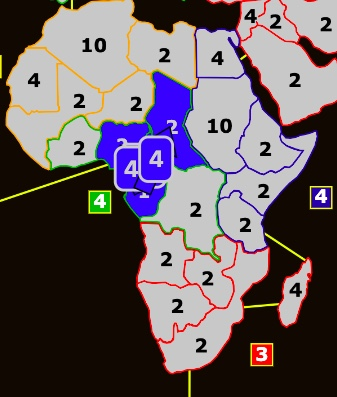
\includegraphics[width=\linewidth, height=9cm]{Images/44wrsplit.jpg}
    \caption{Split attacking with 4 \& 4}
    \label{44wrsplit}
  \end{minipage}
  \hfill
  \begin{minipage}[b]{0.48\linewidth}
    \centering
    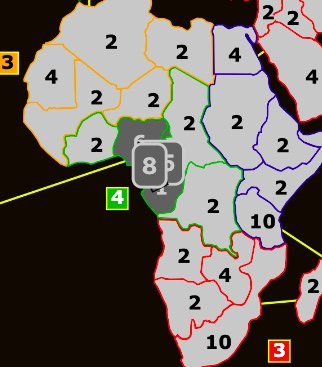
\includegraphics[width=\linewidth, height=9cm]{Images/single8wr.jpg}
    \caption{Single 8 attack}
    \label{single8wr}
  \end{minipage}
\end{figure}

This has a further application when considering the usefulness of leftover armies. Taking into consideration \href{https://www.warzone.com/Forum/149405-trans-attc-percentage-cards?Offset=0}{Frog's Tips}, you'll see in games like \href{https://www.warzone.com/MultiPlayer?GameID=14703564}{this, Turn 1 SEA} and \href{https://www.warzone.com/MultiPlayer?GameID=7926274}{here, Turn 1 East China}, the players go for 3army attacks on Turn 1 attempting to finish their bonuses. If the reason doesn't come intuitively, since the goal is to complete the bonus by the end of T2, a 3attack over the course of two turns captures the bonus 92\% of the time. It boils down to:
\[
\left\{
\begin{aligned}
a1) P(C \land L_{1}) &= 0.8\times0.6 = 0.48 \\[4pt]
a2) P(C \land L_{2}) &= 0.8\times 0.4 = 0.32 \\[4pt]
a3) P(\bar{C} \land L_{1}) &= 0.2 \times 0.6 = 0.12 \\[4pt]
a4) P(\bar{C} \land L_{2}) &= 0.2 \times 0.4 = 0.08
\end{aligned}
\right.
\]
\begin{itemize}
    \item In Scenarios a1, a2, we successfully capture (80\% chance) and have either -1 or -2 attackers.
    \item In Scenario a3, the 3v2 doesn't go our way but we only lost 1 attacker and do not need to deploy another army so as to capture the territory on Turn 2, as for example in this \href{https://www.warzone.com/MultiPlayer?GameID=26746732}{game} in SEA Turn 1.
    \item a3 is the only scenario we don't capture on Turn 1 and need to deploy +1 on Turn 2. 
\end{itemize}


\subsection{Kill-Rates}

We analyzed some sections ago how Kill-Rates are of outmost importance in SR, as the game is deterministic and some attacks are strictly always better. In WR that is and isn't the case. It's a sensitive subject. I have found for example that attacks at multipliers of 5 aren't really worth it. For example \href{https://www.warzone.com/MultiPlayer?GameID=30166708}{here} Octane captures a 3-army neutral with a 4-attack because he wants to maximize his chances to getting to 12 end of T2. If the attack doesn't work (60\% of the time it doesn't work), the 3 army neutrals either kill 2 (90\%) or 3 (10\%) attackers. On the 90\% scenario, Octane can capture that territory with a 2v1 attack without any deployment on T2. Overall this means that if Octane wants to capture that territory with 4 attackers regardless of whether that's on T1 or T2, only 6\% of the time he'd have to deploy +1 T2 (0.6 x 0.1). 
\\
\\
The take-away is that in WR there are a lot of circumstances you will want, deliberately, to attack with something like 14 attackers hoping for the 40\% roll on killing 9 defenders. Or defending with 9 because 9x0.7=6.3 if you sneak a -7 attackers that's awesome. If you have no idea what I'm talking about, revisit Tables \ref{table:attackerResidue} and \ref{table:defenderResidue} as well their corresponding sections.
\\
\\
Regarding the attacker curves, Table \ref{table:attackerResidue_WR}, residue 1 and 3 still give you that 60\% and 80\% shot at one extra kill at no extra cost (like the 3,6,8,11 etc attacks in SR). \textbf{Multiples of 5 give 0 advantage} (besides precision which rarely matters in WR). Residue of 4 gives you a 40\% chance free kill. Attack of 4 in neutral of 3 as we said captures on T1 40\% of the time and on T2 94\% of the time. Residue of 2 you are pushing your luck.

\small
\begin{longtable}{|c|l|c|c|}
\hline
\rowcolor{Baby_Blue}
$r$ (mod 5) & E=0.6,n & Fractional Part & P(+1 extra kill) \\ 
\hline\hline
\endfirsthead
\hline
\rowcolor{Baby_Blue}
$r$ (mod 5) & E=0.6,n & Fractional Part & P(+1 extra kill) \\  \\ 
\hline\hline
\endhead
0 & $3k.0$ & 0 & 0\% (deterministic) \\ 
1 & $3k.6$ & 0.6 & \textbf{60\%} \\
2 & $3k.2$ & 0.2 & 20\% \\
3 & $3k.8$ & 0.8 & \textbf{80\%} \\
4 & $3k.4$ & 0.4 & 40\%  \\
\hline
\caption{Attacker curves 60\% KR, modulo-5, WR}
\label{table:attackerResidue_WR}
\end{longtable}
\normalsize

Regarding the defender curves and Table \ref{table:defenderResidue_WR}, 
\begin{itemize}
    \item The best defender residues statistically are 7>4>1>8>5. 
    \item Defenders of 10 are perfect (good and bad, just 0 variance).
\end{itemize}
But isn't it just so tempting knowing that you can defend with 2 and attack 2 attackers 40\% of the time. Ideally, fit moves for your position. Generally low Fractional Parts are worthwhile when:
\begin{itemize}
    \item The break is fatal to the opponent and the 20\% shot is worth burning extra armies
    \item You would deploy those armies there anyway.
\end{itemize}


\small
\begin{longtable}{|c|l|c|c|}
\hline
\rowcolor{Baby_Blue}
$r$ (mod 10) & E=0.7,n & Fractional Part & P(+1 extra kill) \\ 
\hline\hline
\endfirsthead
\hline
\rowcolor{Baby_Blue}
$r$ (mod 10) & E=0.7,n & Fractional Part & P(+1 extra kill) \\ 
\hline\hline
\endhead
0 & $3k.0$ & 0 & 0\% (deterministic) \\ 
1 & $3k.7$ & 0.7 & \textbf{70\%} \\
2 & $3k.4$ & 0.4 & 40\% \\
3 & $3k.1$ & 0.1 & 10\% \\
4 & $3k.8$ & 0.8 & \textbf{80\%}  \\
5 & $3k.5$ & 0.5 & 50\%  \\
6 & $3k.2$ & 0.2 & 20\%  \\
7 & $3k.9$ & 0.9 & \textbf{90\%}  \\
8 & $3k.6$ & 0.6 & \textbf{60\%}  \\
9 & $3k.3$ & 0.3 & 30\%  \\
\hline
\caption{Defender curves 70\% KR, modulo-10, WR}
\label{table:defenderResidue_WR}
\end{longtable}
\normalsize

Beyond that, the wildest difference between SR and WR comes at n!: n! fronts. Take SR fronts for instance, and the first 22 scenarios in Table \ref{n!_front_SR} (example, a front of 12vs12 where both players attack each other results in 4vs5 (difference 1). This verifies Tables \ref{table:attackerResidue} and \ref{table:defenderResidue} from the SR Kill-Rate section. In fact, in SR 60/70 kill-rates and n!:n! fronts where both players attack each other, the defender will capture back only in 3 occasions. The 5vs5 -> 1vs3 -> 2 capture 1, the 8vs8 -> 2vs4 -> 3 capture 2, and the 15vs15 -> 4vs7 -> 6 capture 4. \textit{(So really in SR just don't do inefficient attacks.)}

\small
\begin{longtable}{|c|c|c|c|c|}
\hline
\rowcolor{Baby_Blue}
Attackers before & Defenders before & Attackers after & Defenders after & Difference \\ 
\hline\hline
\endfirsthead
\hline
\rowcolor{Baby_Blue}
Attackers before & Defenders before & Attackers after & Defenders after & Difference \\ 
\hline\hline
\endhead
2  & 2  & 1 & 1 & 0 \\
3  & 3  & 1 & 2 & 1 \\
4  & 4  & 1 & 2 & 1 \\
5  & 5  & 1 & 3 & 2 \\
6  & 6  & 2 & 3 & 1 \\
7  & 7  & 2 & 3 & 1 \\
8  & 8  & 2 & 4 & 2 \\ \hline
9  & 9  & 3 & 4 & 1 \\ \hline
10 & 10 & 3 & 5 & 2 \\
11 & 11 & 3 & 5 & 2 \\ \hline
12 & 12 & 4 & 5 & 1 \\ \hline
13 & 13 & 4 & 6 & 2 \\
14 & 14 & 4 & 6 & 2 \\
15 & 15 & 4 & 7 & 3 \\
16 & 16 & 5 & 7 & 2 \\
17 & 17 & 5 & 7 & 2 \\
18 & 18 & 5 & 8 & 3 \\ \hline
19 & 19 & 6 & 8 & 2 \\ \hline
20 & 20 & 6 & 9 & 3 \\
21 & 21 & 6 & 9 & 3 \\
22 & 22 & 7 & 9 & 2 \\
\hline
\caption{Attacker-Defender difference in n!:n! front in SR}
\label{n!_front_SR}
\end{longtable}
\normalsize

In WR you can have n!:n! eliminations more often, like \href{https://www.warzone.com/MultiPlayer?GameID=41504555}{here T1} and \href{https://www.warzone.com/MultiPlayer?GameID=40648576}{here T3}. Hell, imagine the 4vs4 scenario which is extremely common. In SR 4vs4, attack of 3 by attacker. 4vs4-> 1vs2 then defender taps into nothing and it drops to 1vs1. In WR the defender can eliminate back \textbf{28\%} of the time. I'm not kidding grab your probabilities handbook and follow along.
\begin{itemize}
    \item 4v4, Attack of 3, first event. 
    \item Attacker has 80\% to kill 2, 20\% to kill 1 defender.
    \item Defender has 80\% chance to kill 3 attackers, 20\% chance to kill 2 attackers.
    \item 4 Scenarios, Joint Probabilities of each:
    \begin{enumerate}
        \item 64\% to end up in a 1vs2 scenario (-3,-2).
        \item 16\% to end up in a 2vs2 scenario (-2,-2).
        \item 16\% to end up in a 1vs3 scenario (-3,-1).
        \item 4\% to end up in a 2vs3 scenario (-2,-1).
    \end{enumerate}
    \begin{enumerate}
        \item In Scenario 1, defender attacks with 1 against 1. If the stars align 18\% of the time you recapture.
        \item In Scenario 2, it's 0\%.
        \item In Scenario 3, defender attacks with 2 against 1. 100\% of the time recapture.
        \item In Scenario 4, defender attacks with 2 against 2. That's 12\% chance you recapture (20\% your 2 attackers establish dominance killing 2 and 60\% the 2 defenders just kill 1 attacker and allow you to spread your armies as stand-guard in the 2 territories)
    \end{enumerate}
    \item Overall chance to get eliminated in a 4vs4 front where both attack each-other at $(0.64 \times 0.18) + (0.16 \times 1) + (0.16 \times 0) + (0.04 \times 0.12) = 0.28$ or 28\%.
\end{itemize}

The issues are not limited to the 4vs4 scenario. I calculated manually the probabilities for 5vs5 and 7vs7, fed the algorithm to chatGPT, verified those 2 and got back the numbers up to 20vs20 below. This aligns with everyone's opinion that in WR you should just build a stack before attacking as losses tend to minimize with bigger army stacks. In fact as you can see, 20vs20 you cannot get eliminated.
\begin{itemize}
    \item 3vs3: 14.40 \%
    \item 4vs4: 28.00 \%
    \item 5vs5: 37.20 \%
    \item 6vs6: 29.60 \%
    \item 7vs7: 35.28 \%
    \item 8vs8: 39.84 \%
    \item 9vs9: 30.80 \%
    \item 10vs10: 24.00 \%
    \item 11vs11: 28.00 \%
    \item 12vs12: 25.60 \%
    \item 13vs13: 8.80 \%
    \item 14vs14: 9.60 \%
    \item 15vs15: 18.00 \%
    \item 16vs16: 12.00 \%
    \item 17vs17: 7.20 \%
    \item 18vs18: 9.60 \%
    \item 19vs19: 9.60 \%
    \item 20vs20: 0 \%
\end{itemize}

Statistically speaking:
\begin{enumerate}
    \item Fronts 3-4 you usually survive, <30\% chance to get erased.
    \item Fronts 5-11 are practically a coin-flip.
    \item Fronts 12-19 Things work in your favour, bigger stacks make it harder for the defender B to counter back and have the army-stand guard to survive.
    \item Above 20, one-turn wipe is mostly impossible (6\% at 22v22, 3\% at 23v23 and 1\% at 29v29).
    \item You can legitimately, get recaptured back if you attack in a 7vs6 scenario first as long as the position becomes 2vs3 (His 6 defenders kill 5 attackers 20\% and your 6 attackers kill 3 defenders 40\% -> 8\% Scenario). From there, as long as they attack you back with 2, kill 2 (20\%), and your 2 defenders kill only 1 (60\%), they get to capture back (8\% chance in this Particular Scenario). Overall chance 0.64\%.
\end{enumerate}
Actual tips for your gameplay:
\begin{enumerate}
    \item Need to reduce variance -> Multiples of 5 for attack, Multiples of 10 for defense.
    \item Need a chance to break -> Add 1-2 armies and the 60\%+ of rolls can give what you need and 14 attackers might just kill 9 defenders 40\ of the time. (Remember for attackers Table \ref{table:attackerResidue_WR}. modulo-4 is 40\% to roll up. modulo-2 is 20\%.)
    \item Small stacks 5-11 -> Add +1 (If your opponent is at n go up to n+1. n can capture back vs n+1 only at 4vs3 and 7vs6), or just move second -> out-delay, or just \textbf{don't attack at all}. 
\end{enumerate}

The conclusion after this completely pointless, unnecessarily lengthy and fruitless explanation is that WR fits under \textit{predictable variance}. You can compute the odds and decide based on that. Or you can completely veto the templates in Tables \ref{table:wr_rmo_cards_trimmed} and \ref{table:wr_cyclic_cards_trimmed}.  WR comes with a couple of significant advantages over SR in that a) it will practically never result in a draw and b) it can (and often will) be harder to find an optional set of moves for your position (rarer so picks). You have to build an intuition on figuring out how to best  use all your leftovers in coordination, as calculating is tedious. The enormous disadvantage comes at how sometimes lady luck determines the outcome of the game, and not you. You can play every single correct move, and still lose. But the moves themselves are less clear than SR's gameplay, especially in the 2025 landscape where players have long forgotten how to play WR and find joy mostly in SR. 